All results should be reported with k-fold cross validation accuracies, using
standard deviation in the folds as an uncertainty estimate.
\begin{itemize}
  \item Logistic regression results 
  \item Dense network results
  \item CNN results
  \item ? - Pretrained network results
  \item Project model - Attempt to reproduce results
\end{itemize}
\section{Classification}
\subsection{Simulated data}
Classification results using models within a range of complexities are presented in table \ref{tab:classification-sim}.
Reported figures are performance on test set (NOT YET THO)
\begin{table}
  \centering
  \begin{tabular}{|l|c|c|c|}
    Model     & f1max & f1min & f1avg \\
    \hline
    Logistic  &       &       &   \\
    DNN       &       &       &   \\
    CNN       &       &       &   \\
  \end{tabular}
  \caption{Table of classification performance for a range of models trained on simulated data.}
  \label{tab:classification-sim}
\end{table}




\begin{figure}
\centering
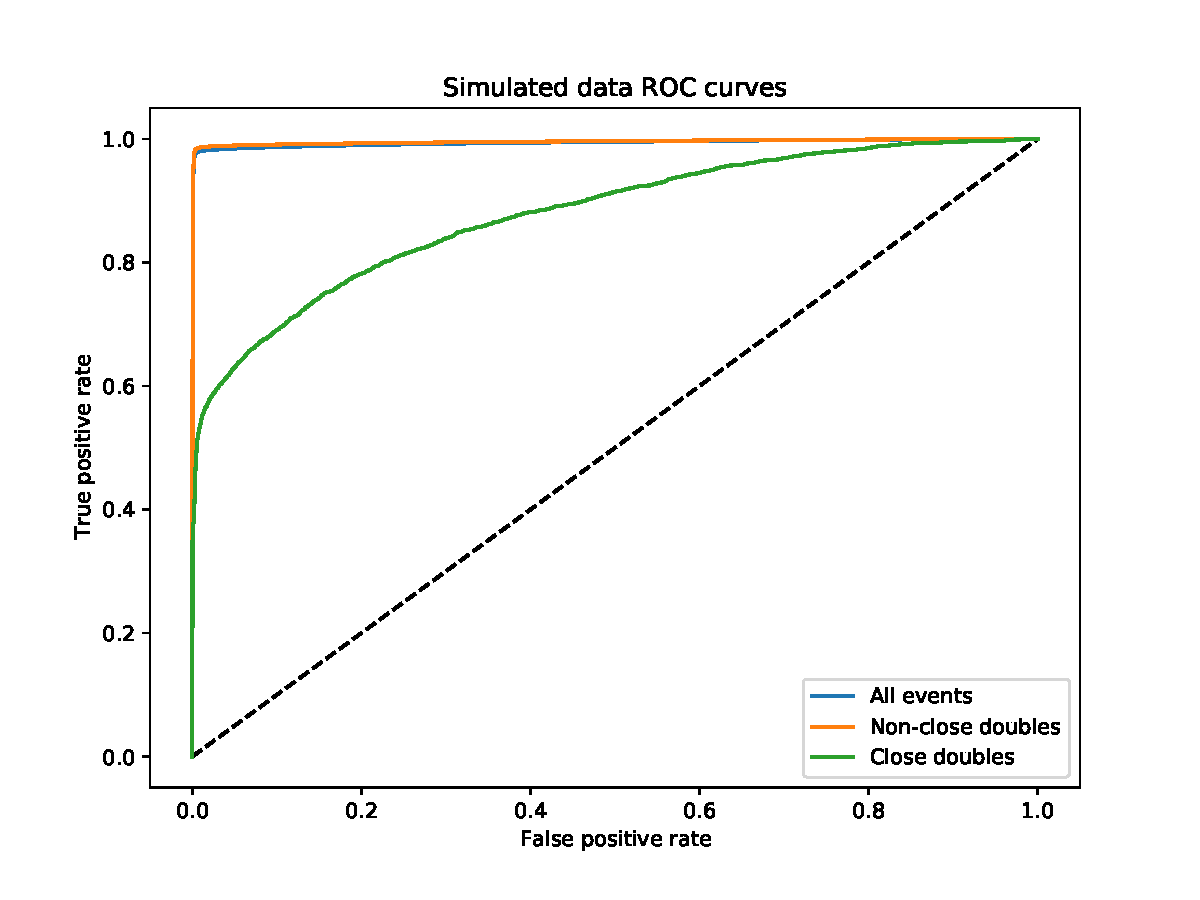
\includegraphics[width=0.8 \textwidth]{chapters/results/figures/roc_simulated.pdf}
\caption[Titletext]{generic text}\label{fig:roc_simulated}
\end{figure}

\subsection{Regression}
Same approach as for classification.
\begin{itemize}
  \item ? - Linear approach?
  \item ? - Dense network
  \item ? - CNN
\end{itemize}
\subsubsection{Position}
\subsubsection{Energy}
\subsection{Experimental data}
\subsection{Classification}
\subsection{Regression}
\subsubsection{Position}
\subsubsection{Energy}
